\subsection{Rangefinder Testing}
The URG-04LX scanning laser rangefinder requires an external 5V power source connection. With the power connected and the device on, the device is ready and waiting for communication.

\subsubsection{Testing via the Data Viewing Tool}
The URG-04LX has a data viewing tool which is a useful application by Hokuyo Automatic Co. that can be used to view, record, and replay the device's data. To use this tool the device must be plugged into a computer via its USB port. Figure \ref{URGBenriStandard_pic} below shows a screen capture of the application recording data captured by the rangefinder.

\begin{figure}[H]
	\centerline{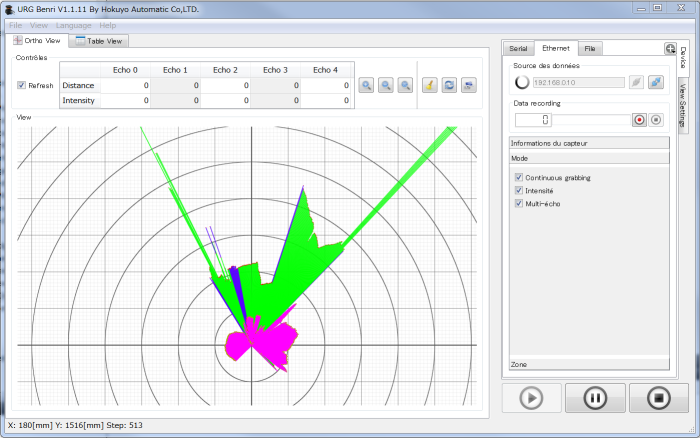
\includegraphics[width=1\textwidth]{UrgBenri_screenshot.png}}
	\caption{Screen Capture of the URG-04LX Data Viewing Tool \cite{URGBenriStandard_ref}}
	\label{URGBenriStandard_pic}
\end{figure}

Note that the start point of 0, end point of 768, and dead zone align to that shown in Figure \ref{rangefinder_fov}. For this project the data viewing tool was used to verify our project's data processing functionality.

\subsubsection{Command Testing}
In addition to the data viewing tool, we were able to test the rangefinder's commands by connecting it to a laptop via its USB port. We used PuTTy, a serial console application, to communicate with the rangefinder. Figure \ref{rangefinder_putty} shows the data transfer via PuTTy between a laptop and the rangefinder. Note that PuTTy only shows data received, and that the rangefinder always echoes back the command that it receives.

\begin{figure}[H]
	\centerline{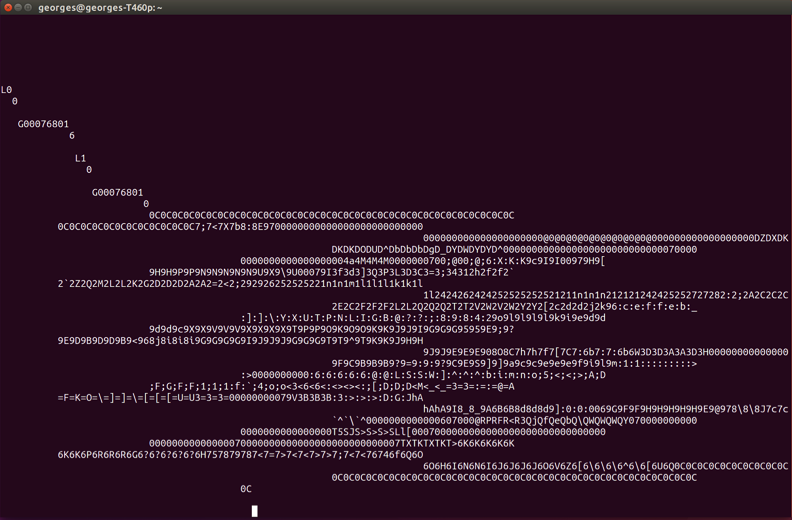
\includegraphics[width=1\textwidth]{rangefinder_putty.png}}
	\caption{Rangefinder Communication Test via PuTTy}
	\label{rangefinder_putty}
\end{figure}

The figure above shows four communication sequences. The first is the laser illumination command 'L0\textbackslash{}n'. Since the laser defaults on, this command turned the laser off. The rangefinder responded to this command first with the echo 'L0\textbackslash{}n', and then with '0', indicating success. The second command is our data acquisition command 'G00076801\textbackslash{}n'. The rangefinder responded with '6', indicating an error code, which was caused by the laser being off. The third command is the laser illumination command again, which turns on the laser. The rangefinder's response was '0' again, indicating success. The last command shown is the data acquisition command again. The rangefinder's response begins with '0', indicating success, followed by the distance data block. The data block consists of 768 points, specified by the data acquisition command. Each data point consists of two characters \cite{urg04lx_datasheet}. By communicating with the rangefinder via PuTTy, we were able to observe the rangefinder's behavior and confirm the data acquisition command functions properly. This testing also verified that communication via the rangefinder's USB port was working.

\subsubsection{Communication via USB On-The-Go (OTG)}
With communication via the rangefinder's USB port working, we decided to continue with this mode of communication. The ZedBoard supports USB On-The-Go (OTG) which is a specification that allows USB devices to act as a host for other USB devices \cite{usb-otg}. With USB OTG, a device can choose to act as a peripheral or a host if necessary. For the purpose of this project, the ZedBoard will act as the host by initiating communication with the rangefinder. Enabling USB OTG can be done in the Zynq7 Processing System and controlled through the PS. The rangefinder's laser illumination command was chosen to be transmitted from the ZedBoard to test the communication. This command was chosen because when received, the status LED on the rangefinder blinks until the laser is turned back on, which is a simple way of verifying successful communication. In addition, when a command is transmitted via UART from the ZedBoard, its TX LED flashes. A fully successful transaction would observe the ZedBoard's TX LED flashing and then the status LED on the rangefinder blinking.
\par
The ZedBoard was programmed, the rangefinder was turned on, and the two devices were connected by a standard micro-USB to mini-USB cable. The ZedBoard transmitted the command, as signified by the blink of the TX LED. However the rangefinder did not acknowledge the command; its status LED was staying lit signifying the laser was on. Due to this failure\footnote{This communication failure was most likely due to the lack of necessary hardware, as USB OTG requires an adapter that controls which device will be hosting the communication. Without this adapter, both USB devices will act as a peripheral, and neither will initiate communication \cite{usb-otg}.}, using USB OTG was not implemented. Instead the methodology described in Section \ref{sssec:rangefinder_communication} was implemented.

\subsubsection{Communication via Pmod}
Once we decided not to continue with USB OTG, we routed the UART signals to a Pmod connector, described in Section \ref{sssec:rangefinder_communication}. To make sure that UART via Pmod was functioning correctly, the transmit pin was measured with an oscilloscope. The laser illumination command "L0\textbackslash{}n" was transmitted and observed indicating success, as shown in Figure \ref{laser_illumination}. Note that this is a TTL signal.

\begin{figure}[H]
	\centerline{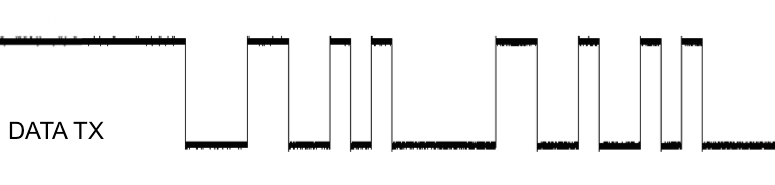
\includegraphics[width=.7\textwidth]{laser_illumination_labeled.png}}
	\caption{Laser Illumination Command TTL Oscillogram}
	\label{laser_illumination}
\end{figure}

The RS-232 to TTL converter with the attached breakout board was attached to the ZedBoard. The converter's V\textsubscript{CC} and GND were connected to the ZedBoard Pmod's respective V\textsubscript{CC} and ground pins. When these pins were connected, the converter's power LED turned on. In addition, the converter's RX and TX pins were connected to the ZedBoard's respective TX and RX pins. The breakout board's TX pin was measured on the oscilloscope to observe the resultant RS-232 waveform. However when the command was transmitted from the ZedBoard, there was no change on the oscilloscope. We disconnected the converter's TX and RX pins and reconnected them such that the converter's RX and TX pins were connected to the ZedBoard's respective RX and TX pins. The laser illumination command was re-transmitted and the waveform in Figure \ref{rangefinder_rs232} was observed on the oscilloscope. The oscillogram shows a waveform from +6V to -6V, which is a valid RS-232 signal.

\begin{figure}[H]
	\centerline{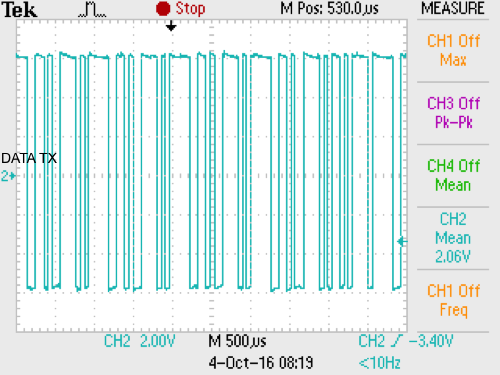
\includegraphics[width=.7\textwidth]{rangefinder_rs232_label.png}}
	\caption{Laser Illumination Command RS-232 Oscillogram}
	\label{rangefinder_rs232}
\end{figure}

With the communication functioning properly, the rangefinder's RX and TX were connected to the breakout board's respective TX and RX pins, and the laser illumination command was transmitted from the ZedBoard. The rangefinder's status LED started blinking, signifying that it received the laser illumination command and the laser was turned off. This test's success indicates that the rangefinder's communication is completely successful.

\subsubsection{PS-PL Testing}
Once UART communication was verified, the next step was to test the PS-PL communication. In order to test the communication, UART was reconfigured in the processing system to be routed to USB UART.
\par
PL to PS communication was tested first, by using a PL button press to initiate a UART transfer. With UART routed to USB UART, the TX LED will flash when data is transmitted. In the PL, BTNR was used as an input and was wired into the AXI's output register, $reg\textunderscore{}data\textunderscore{}out$, as $slv\textunderscore{}reg0$, as seen on line 368 of the custom IP's instantiated file located in Appendix \ref{customIPaxi}. In the PS, the data was read from the AXI bus by pointing to the address in memory where the PL's output register, $slv\textunderscore{}reg0$, is located. This address can be found in the SDK in the $system.dhf$ file, which contains the hardware platform specifications. The base address is the cell with the same name as the custom IP. For this project, the base address was 43C00000\textsubscript{16}. Since $slv\textunderscore{}reg0$, the first of the four designated memory registers, was used there does not need to be any address offset. Reading from the PL was implemented on line 30 of the PS, shown in Appendix \ref{ps_code}, by using Xilinx's function $Xil\textunderscore{}In32$ to read the data from the memory address that is $baseaddr\textunderscore{}p$\footnote{This could also have been accomplished by using a pointer to read the data from the memory address that is $baseaddr\textunderscore{}p$.}. Once the setup was complete, the ZedBoard was programmed and connected to a serial console. BTNR was pressed and the TX LED lit up, indicating that PL to PS communication was functioning properly.
\par
PS to PL communication was tested next per use of the VGA screen. For this test, the PL transmit signal will be received and then the PS will wait for 768 data points to be received, just as if the rangefinder were connected. Since UART was routed to USB UART, the ZedBoard can communicate with a serial console. Through the serial console, rangefinder communication can be simulated by inputting a block of rangefinder data. The data will be written to the PL one data point at a time by writing to $slv\textunderscore{}reg1$, as on line 239 of the custom IP's instantiated file located in Appendix \ref{customIPaxi}. This register is located one memory register from the base address of the custom IP because it is the second of the four designated memory registers. The function $Xil\textunderscore{}Out32$ was first tested but no results were observed, so a pointer was used to write to the base address offset by one memory register. This is seen on line 198 of the PS, in Appendix \ref{ps_code}. The data written to $slv\textunderscore{}reg1$ was the distance data point, a data valid flag, and the rangefinder step. These were manipulated to fit into one 32-bit integer by shifting each to a unique bit location of a buffer, $data\textunderscore{}enable\textunderscore{}step$.
\par
To test data accuracy in addition to PS to PL communication, the block of data sent from the serial console will be constant. With data constant across all steps of the rangefinder's field of view, $270^\circ$ of a circle should be drawn around the rangefinder on the VGA screen. With the VGA module set up and the rangefinder data processing ready to be tested, the ZedBoard was programmed. When BTNR was pushed, an image similar to Figure \ref{badCircle} was observed on the VGA screen with the red dot being the device and the black lines being the rangefinder's distance data.

\begin{figure}[H]
	\centerline{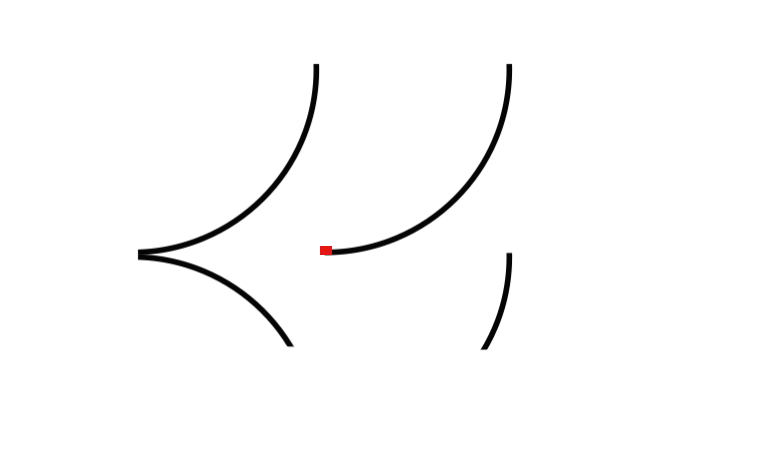
\includegraphics[width=.5\textwidth]{badCircle.png}}
	\caption{PS to PL Communication Test with Constant Data}
	\label{badCircle}
\end{figure}

Although a circle was not observed, this test confirmed the PS to PL communication was functioning properly. The shape appears to look like four quadrants of a circle in the wrong direction. Since the lines seem semi-circular, the polar-to-rectangular transformation seems to be successful, too. The problem is a minor sign issue with the rangefinder's data processing in the PL. The signs in each necessary quadrant were fixed and the test was repeated with Figure \ref{goodCircle} observed on the VGA screen.

\begin{figure}[H]
	\centerline{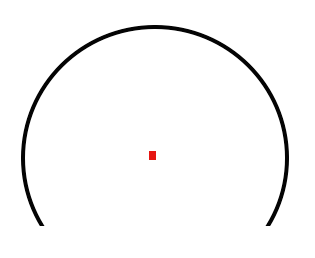
\includegraphics[width=.4\textwidth]{goodCircle.png}}
	\caption{PS to PL Communication with Constant Data and Edited Data Processing}
	\label{goodCircle}
\end{figure}

With the PS-PL communication and rangefinder data processing functioning perfectly, the rangefinder can be attached and tested.

\subsubsection{Data Testing}
UART was re-routed to the PS Pmod in order to test the entire rangefinder implementation. The rangefinder was powered by the lab bench power supply and was connected on the RS-232 breakout side of the RS-232 to TTL converter, with the ZedBoard connected to the TTL side. The ZedBoard was connected to the VGA screen, and then was programmed. BTNR was pushed to initiate the UART transfer and Figure \ref{first} shows the VGA output.

\begin{figure}[H]
	\centerline{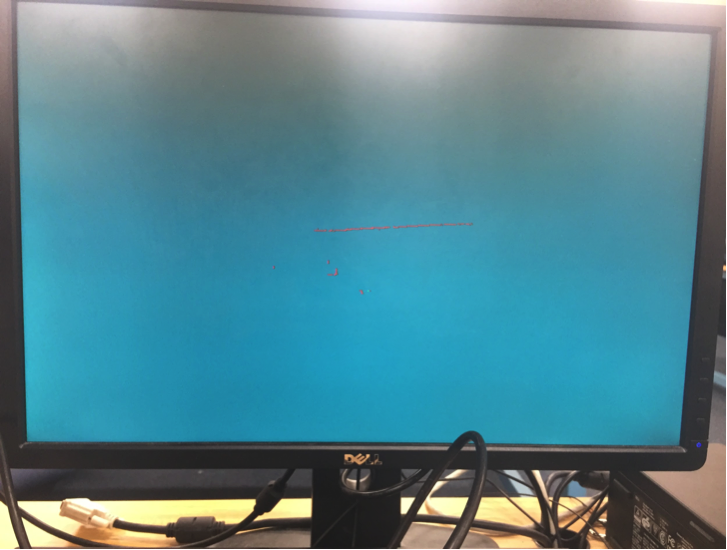
\includegraphics[width=.7\textwidth]{first.png}}
	\caption{Rangefinder Data Observed on VGA Screen}
	\label{first}
\end{figure}

Next BTNR was pushed again to start another data transfer, but there was no observed functionality. The button was held down until the subsequent data transfers in Figure \ref{subsequent} were observed on the VGA screen.

\begin{figure}[H]
	\centerline{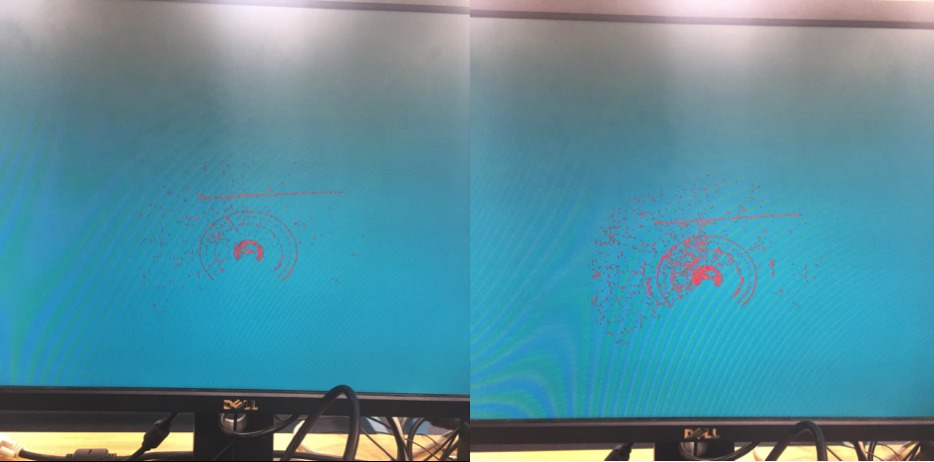
\includegraphics[width=.9\textwidth]{subsequent.jpg}}
	\caption{Subsequent Rangefinder Data Observed on VGA Screen}
	\label{subsequent}
\end{figure}

In the SDK the PS was not accounting for enough data points. When the rangefinder receives a command from the ZedBoard it echoes back the command. This is used as a test to ensure data accuracy. Since not enough data was being accounted for, the extra data was writing into the next data transfer's input echo buffer. As a result, the echo received from the rangefinder did not match the command transmitted and the rest of the data was garbage. The PS was edited to account for all of the data points and the data transfers were able to be triggered every time BTNR was pressed.
\par
Figure \ref{labtest1} shows a test of the rangefinder where its output is compared to the objects around it.

\begin{figure}[H] 
	\begin{subfigure}{1\textwidth}
	\centering
		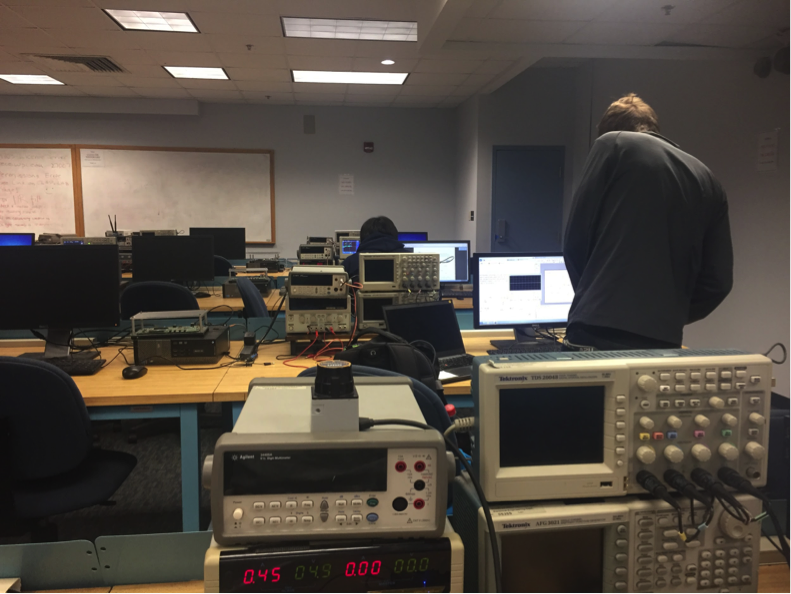
\includegraphics[width=0.75\linewidth]{labtest1_1.png}
		\caption{Lab at WPI}
		\label{lab1}
	\end{subfigure}
	\begin{subfigure}{1\textwidth}
	\centering
		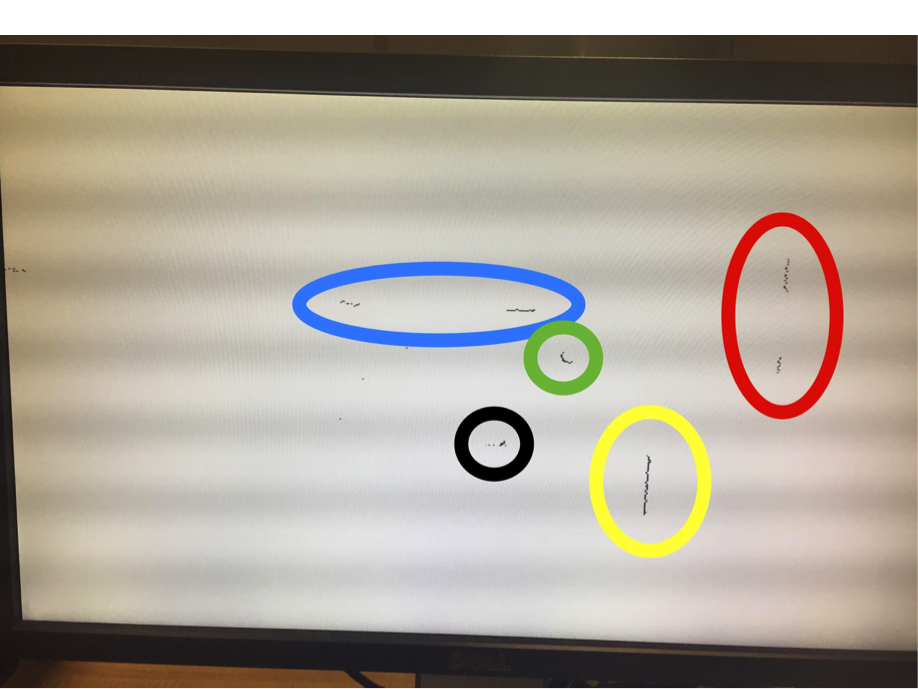
\includegraphics[width=0.75\linewidth]{labtest1_2.png}
		\caption{2D Rangefinder "Floorplan" of Lab at WPI}
		\label{floorplan1}
	\end{subfigure}
	\caption{First Lab Test of Rangefinder Functionality}
	\label{labtest1}
\end{figure}

In Figure \ref{labtest1}(\subref{floorplan1}), the data points in the black circle represent the rangefinder and the lab bench oscilloscope that is right next to it. The straight line circled in yellow is the wall directly to the right of the lab bench. The lines circled in red show the lab doorway with the door open. The data in the green circle is the student in Figure \ref{labtest1}(\subref{lab1}), and the lines in blue are the oscilloscopes and computers in front of the rangefinder.
\par
Next, the screen was cleared, the rangefinder was rotated $180^\circ$, and the process was repeated.

\begin{figure}[H] 
	\begin{subfigure}{1\textwidth}
	\centering
		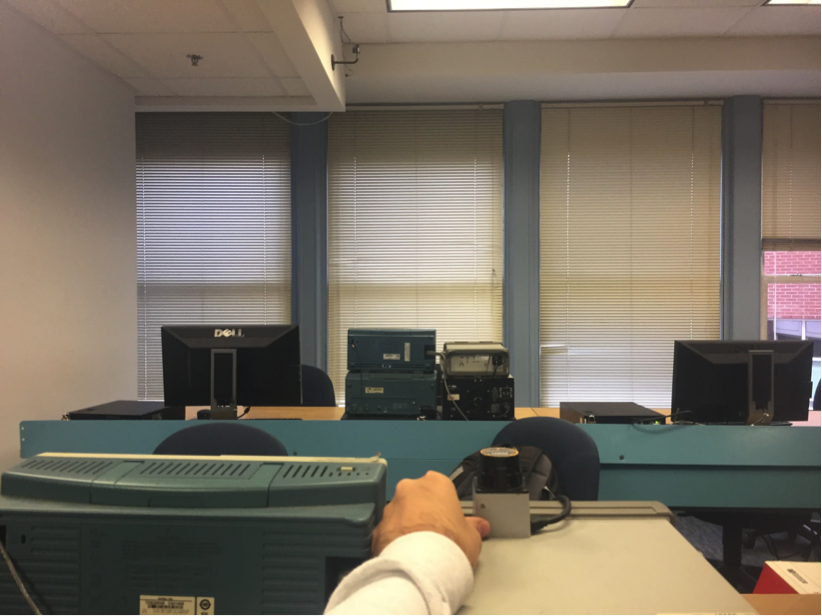
\includegraphics[width=0.75\linewidth]{labtest2_1.png}
		\caption{Lab at WPI with $180^\circ$ Change of Orientation}
		\label{lab2}
	\end{subfigure}
	\begin{subfigure}{1\textwidth}
	\centering
		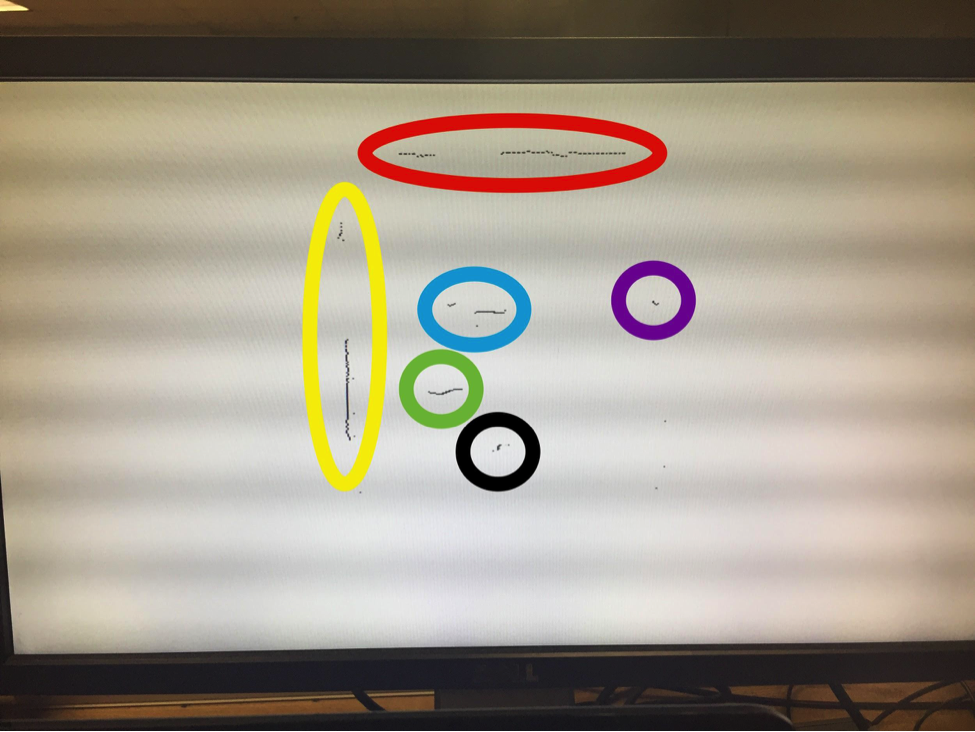
\includegraphics[width=0.75\linewidth]{labtest2_2.png}
		\caption{2D Rangefinder "Floorplan" of Lab at WPI with $180^\circ$ Change of Orientation}
		\label{floorplan2}
	\end{subfigure}
	\caption{Second Lab Test of Rangefinder Functionality}
	\label{labtest2}
\end{figure}

In Figure \ref{labtest2}(\subref{floorplan2}) the black circle is around the rangefinder, the yellow is circling the wall, and the blue is circling the computer and oscilloscope. The green is circling my body while the rangefinder's data capture was being triggered\footnote{Note that I am not shown in Figure \ref{labtest2}(\subref{lab2}) because I moved in order to take the photo.}. The red is circling the windows, and the purple is circling a support beam in the middle of the lab.
\par
Next, the screen was cleared once more. The rangefinder was moved to the first orientation once more to capture data, and then was rotated to the second orientation without clearing the screen. Figure \ref{resultant} shows the resultant VGA output.

\begin{figure}[H]
	\centerline{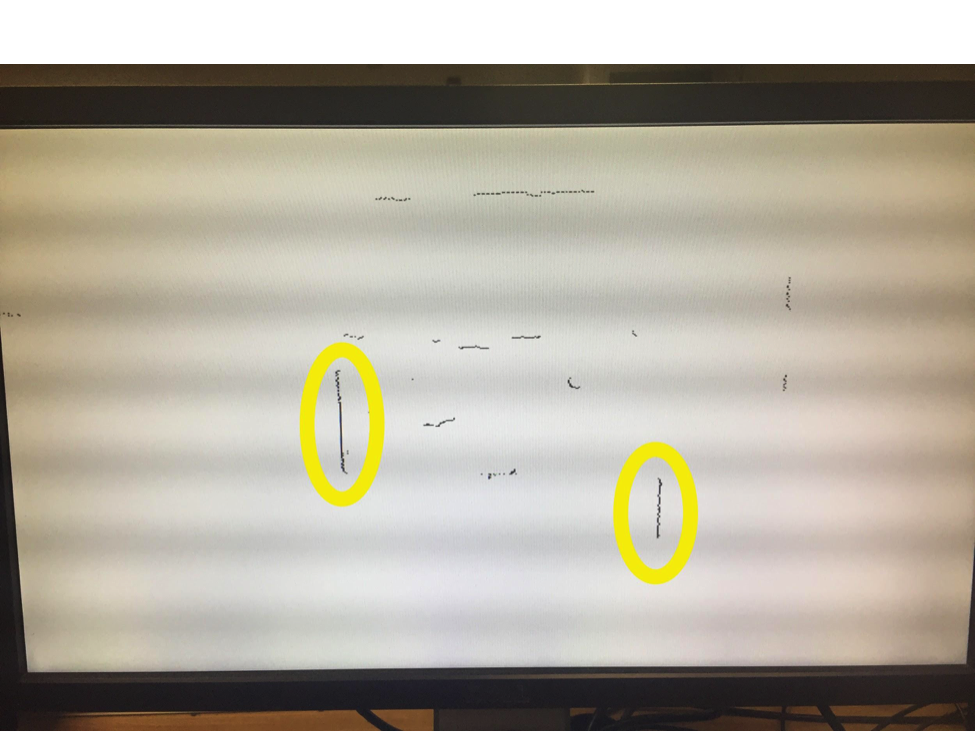
\includegraphics[width=.8\textwidth]{resultant.png}}
	\caption{Two Rangefinder "Floorplan" Captures of Lab with $180^\circ$ Offset}
	\label{resultant}
\end{figure}

Both rangefinder data captures were triggered successfully and without loss of data. Despite the $180^\circ$ change of orientation, both data captures were overlaid on top of each other. Note that the walls circled in yellow are actually the same wall. This issue can be resolved by incorporating the IMU's rotational data. With the IMU's rotational data used to offset the direction of the device, 2D floorplan will accurately reflect the location of objects.




